\chapter{Caratterizzazione di Dati Misurati}
Resi noti una serie di dati misurati, quello che si vuole andare a fare è trovare un modello statistico che mi permetta di avere un'approssimazione valida di tali dati. Ci sono varie tipologie di tecniche e di approcci. Per grandi quantità di dati si farà un utilizzo massiccio della \textbf{Statistica inferenziale}, che comprende tutta una serie di metodi che permettono di andare a stimare un modello quantò più opportuno possibile ai dati che si stanno andando ad analizzare

\subsection{Media, Mediana e Moda}
Dato un insieme di dati, si possono andare a valutare 3 valori principali (e scalari), che ci permettono di approssimare (in maniera grossolana), la nostra distribuzione di dati (rappresentabile, anche, mediante un istogrammma). I valori a cui si fa riferimento sono:
\begin{itemize}
    \item \textbf{Media}: Media statistica di tutti i valori che si sta andando a considerare. Se si ha un set di valoi \(X = (x_1,x_2,\dots,x_n)\), allora definiamo come media:
    \[
    \overline{X} = \frac{1}{n}\sum_{i=1}^{n}x_i
    \]
    La media, però, non tiene conto dell'asimmetria dei dati (skewness), quindi se ad esempio un sistema ha dei tempi di ripsosta sempre stabili, e poi, un singolo caso di tempo di risposta lungo, potrebbe avere la stessa media di un sistema che ha mediamente tempi di risposta più lunghi (molto sensibile ad eventuali comportamenti limite)
    \item \textbf{Mediana}: La mediana di un set di valori \(X = (x_1,x_2,\dots,x_n)\) è data dalla selezione del valore centrale del set di valori ordinati. Per capire, si ordina il set di valori \(X\) e poi si seleziona l'elemento presente in \(\left\lfloor\frac{n}{2}\right\rfloor\). Ciò però presenta un problema, se il numrero di valori è dispari allora io seleziono l'unica posizione centrale presente (es. Se ho 3 elementi seleziono 1), mentre se ho un valore pari devo trovare un modo con cui scegliere quale elemento considerare, pertanto, essendo due i valori centrali, se ne fa la media (es. se ho 4 elementi, farò la media del valore in posizione 1 ed in posizione 2). La mediana a differenza della media viene presa direttamente dai valori reali e non calcolata considerando tutti i valori, ciò gli permette di essere più resistente agli outlier e sopratutto a distribuzioni asimettriche (resistente alla skewness)
    
    \item \textbf{Moda}: La moda rappresenta il valore più probabile all'interno di una distribuzione (quello presentato più volte). Di conseguenza tiene conto del picco presente nell'istrogramma. Il problema della moda è che può non esistere (caso di distribuzioni uniformi), oppure può assumere più di un valore (immaginare una distribuzione bi-gaussiana). Nonostante le considerazioni precedenti, la media è totalmente immune agli outlier (vedo solo il più probabile), e mi permette di evitare anche le ambiguità di una particolare distribuzione
\end{itemize}

\begin{info}
Nella descrizione dei parametri precedenti si è parlato di asimettrie dei dati (skewness dei dati), tale valore per piccole quantità di campioni può essere approssimato con la formula:
\[
skewness = \frac{y_{max}}{y_{min}}
\]
Da tale formula comprendo che più il valore è alto e più i dati sono "asimettrici". Ma tale considerazione è più corretta quanto più è piccola la quantità di campioni che sto andando a considerare 
\end{info}


Un semplice criterio per decidere quale tipologia di metrica utilizzare è quella mostrata in figura [\ref{img:criterio-media-mediana}]

\begin{figure}[h]
\centering
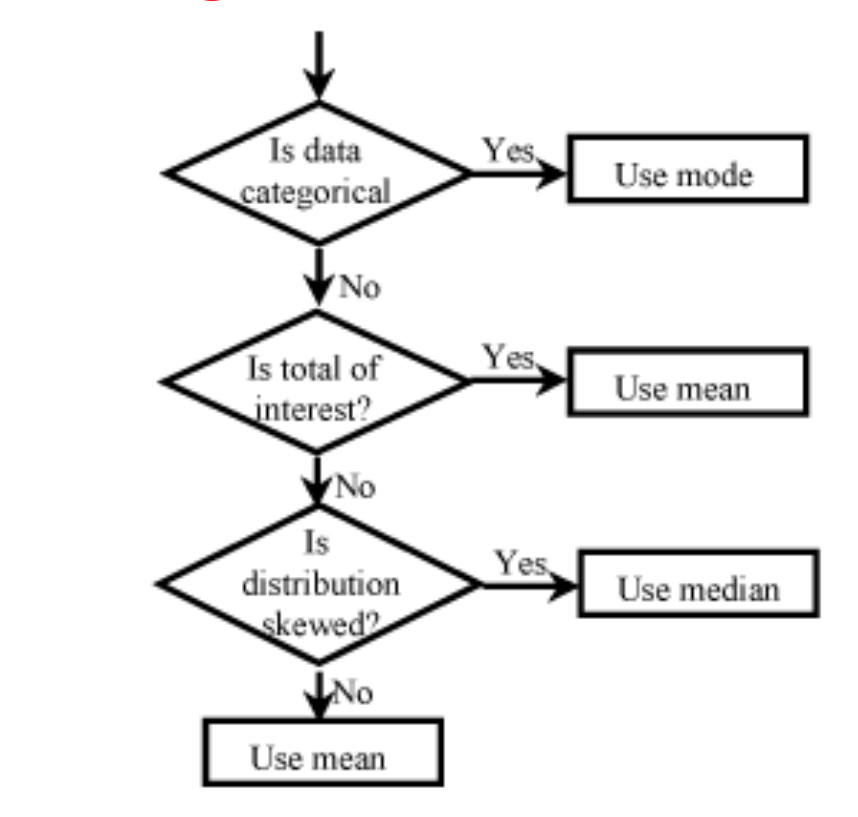
\includegraphics[width=.5\textwidth]{img/criterio-media-mediana.png}
\caption{Semplice schema di un criterio per la scelta della metrica da utilizzare}\label{img:criterio-media-mediana}
\end{figure}

I valori descritti, oltretutto, possono essere ottenuti osservando anche la distribuzione dei dati mediante degli istogrammi di occorrenza. In questo modo è anche più facile campire quale metrica sia meglio utilizzare.

\begin{figure}[H]
\centering
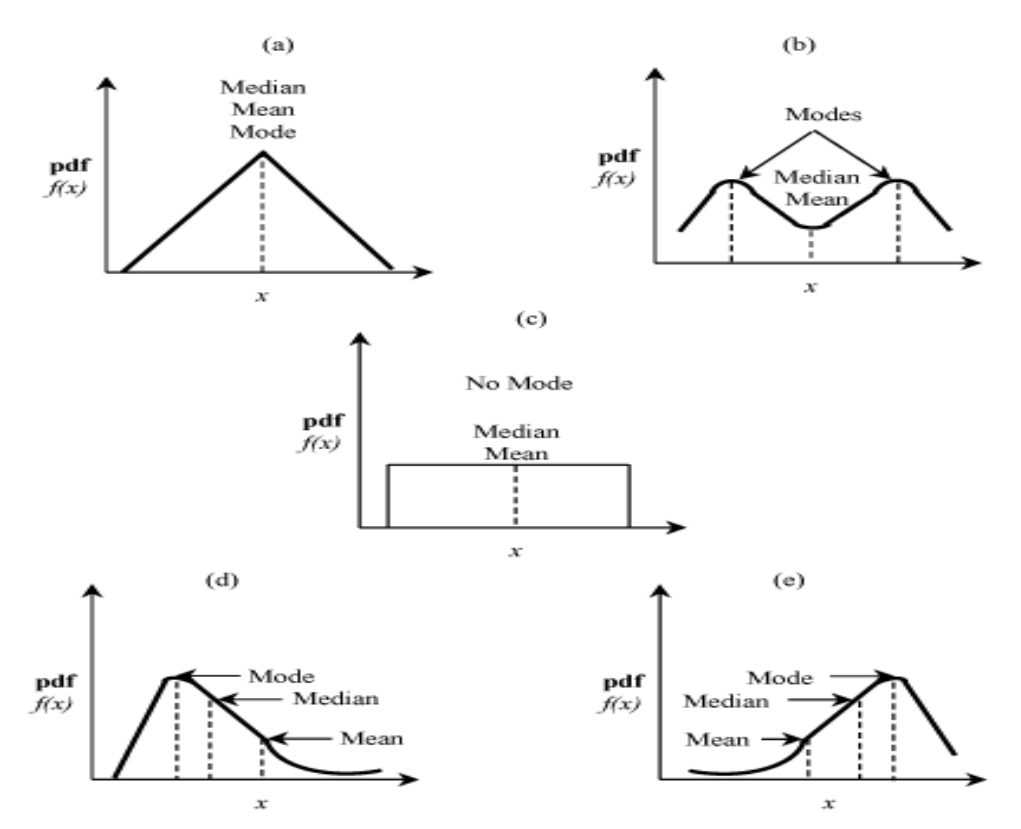
\includegraphics[width=.5\textwidth]{img/grafici-media-mediana.png}
\caption{Grafici illustrativi dei parametri discussi}\label{img:grafici-media-mediana}
\end{figure}

\subsection{Indici di dispersione}
Andare ad approssimare una distribuzione di valori con un singolo valore non basta, tale informazione non mi permette di considerare anche la \textbf{variabilità} che i dati possono avere nel tempo.
Uno strumento utile per avere un'idea della variabilità, sono gli \textbf{indici di dispersione}. Tra le metriche più utilizzate possiamo trovare:
\begin{itemize}
\item \textbf{Range}: Il range è un parametro molto basilare che viene calcolato come: \(v_{max} - V{min}\). Tale metrica, per quanto semplice, è anche molto poco resistente agli outlier
\item \textbf{Varianza campionaria (o deviazione standard)}: Tale parametro è strettamente calcolato dai dait e dipende dalla loro distribuzione
\item \textbf{10- e -90 Percentile}: Prendendo una distribuzione di dati si vanno a considerare due valori:
\begin{itemize}
    \item \textbf{\(P10\)}: Valore dei dati sotto il quale cade il 10\% dei dati considerati
    \item \textbf{\(P90\)}: Valore dei dati sotto il quale cade il 90\% dei dati considerati (quindi solo il restante 10\% è maggiore)
\end{itemize}
Si definisce poi come indice di dispersione il range calcolato su tali valori: \(range = P90-P10\). Se vediamo tali valori in riferimento alla pdf dei dati (il loro istogramma) e alla CDF. Si ha che per calcolare il valore P90 e P10, vado a valutare il valore della CDF in base al percentile ricercato (\(F(x_p) = 0.10\) o \(0.90\)), oppure, nel caso della pdf vado a calutare l'integrale (guardare la relazione tra CDF e pdf)\(\left [\int_{-\infty}^{x_p}f(x)dx = 0.10 | 0.90\right ]\). Il percentile solitamente può essere chiamato anche \textbf{quartile}. La differenza sta nella notazione, per il quartile si dice \(0.1\)-quartile (\(\alpha\)-quartile), mentre il percentile si esprime come 10-percentile (\(100*\alpha\)-percentile). Per stimare tali valori su un insieme di dati discreto (quindi non distribuzioni continue su cui effettuare integrali o derivate), posso andare ad effettuare, prima un ordinamento e poi a selezionare uno specifico valore in base alla \(\alpha\) scelta. Precisamente si va a selezionare il valore in posizione: \([(n-1)*\alpha + 1]\)

\item \textbf{Semi Inter-Quartile Range}:

\end{itemize}